
\documentclass[letterpaper,hide notes,xcolor={table,svgnames},pdftex,10pt]{beamer}
\def\showexamples{t}


%\usepackage[svgnames]{xcolor}

%% Demo talk
%\documentclass[letterpaper,notes=show]{beamer}

\usecolortheme{crane}
\setbeamertemplate{navigation symbols}{}

\usetheme{MyPittsburgh}
%\usetheme{Frankfurt}

%\usepackage{tipa}

\usepackage{hyperref}
\usepackage{graphicx,xspace}
\usepackage[normalem]{ulem}
\usepackage{multicol}
\usepackage{amsmath,amssymb,amsthm,graphicx,xspace}
\newcommand\SF[1]{$\bigstar$\footnote{SF: #1}}

\usepackage[default]{sourcesanspro}
\usepackage[T1]{fontenc}
\usepackage[scaled]{beramono}
\usepackage{tikzpagenodes}

\newcounter{tmpnumSlide}
\newcounter{tmpnumNote}


% old question code
%\newcommand\question[1]{{$\bigstar$ \small \onlySlide{2}{#1}}}
% \newcommand\nquestion[1]{\ifdefined \presentationonly \textcircled{?} \fi \note{\par{\Large \textbf{?}} #1}}
% \newcommand\nanswer[1]{\note{\par{\Large \textbf{A}} #1}}


 \newcommand\mnote[1]{%
   \addtocounter{tmpnumSlide}{1}
   \ifdefined\showcues {~\tiny\fbox{\arabic{tmpnumSlide}}}\fi
   \note{\setlength{\parskip}{1ex}\addtocounter{tmpnumNote}{1}\textbf{\Large \arabic{tmpnumNote}:} {#1\par}}}

\newcommand\mmnote[1]{\note{\setlength{\parskip}{1ex}#1\par}}

%\newcommand\mnote[2][]{\ifdefined\handoutwithnotes {~\tiny\fbox{#1}}\fi
% \note{\setlength{\parskip}{1ex}\textbf{\Large #1:} #2\par}}

%\newcommand\mnote[2][]{{\tiny\fbox{#1}} \note{\setlength{\parskip}{1ex}\textbf{\Large #1:} #2\par}}

\newcommand\mquestion[2]{{~\color{red}\fbox{?}}\note{\setlength{\parskip}{1ex}\par{\Large \textbf{?}} #1} \note{\setlength{\parskip}{1ex}\par{\Large \textbf{A}} #2\par}\ifdefined \presentationonly \pause \fi}

\newcommand\blackboard[1]{%
\ifdefined   \showblackboard
  {#1}
  \else {\begin{center} \fbox{\colorbox{blue!30}{%
         \begin{minipage}{.95\linewidth}%
           \hspace{\stretch{1}} Some space intentionally left blank; done at the blackboard.%
         \end{minipage}}}\end{center}}%
         \fi%
}



%\newcommand\q{\tikz \node[thick,color=black,shape=circle]{?};}
%\newcommand\q{\ifdefined \presentationonly \textcircled{?} \fi}

\usepackage{listings}
\lstset{basicstyle=\footnotesize\ttfamily,
	breaklines=true,
	aboveskip=15pt,
  	belowskip=15pt,
	frame=lines,
	numbers=left, basicstyle=\scriptsize, numberstyle=\tiny, stepnumber=0, numbersep=2pt
}

\usepackage{siunitx}
\newcommand\sius[1]{\num[group-separator = {,}]{#1}\si{\micro\second}}
\newcommand\sims[1]{\num[group-separator = {,}]{#1}\si{\milli\second}}
\newcommand\sins[1]{\num[group-separator = {,}]{#1}\si{\nano\second}}
\sisetup{group-separator = {,}, group-digits = true}

%% -------------------- tikz --------------------
\usepackage{tikz}
\usetikzlibrary{positioning}
\usetikzlibrary{arrows,backgrounds,automata,decorations.shapes,decorations.pathmorphing,decorations.markings,decorations.text,decorations.pathreplacing}

\tikzstyle{place}=[circle,draw=blue!50,fill=blue!20,thick, inner sep=0pt,minimum size=6mm]
\tikzstyle{transition}=[rectangle,draw=black!50,fill=black!20,thick, inner sep=0pt,minimum size=4mm]

\tikzstyle{block}=[rectangle,draw=black, thick, inner sep=5pt]
\tikzstyle{bullet}=[circle,draw=black, fill=black, thin, inner sep=2pt]

\tikzstyle{pre}=[<-,shorten <=1pt,>=stealth',semithick]
\tikzstyle{post}=[->,shorten >=1pt,>=stealth',semithick]
\tikzstyle{bi}=[<->,shorten >=1pt,shorten <=1pt, >=stealth',semithick]

\tikzstyle{mut}=[-,>=stealth',semithick]

\tikzstyle{treereset}=[dashed,->, shorten >=1pt,>=stealth',thin]

\usepackage{ifmtarg}
\usepackage{xifthen}
\makeatletter
% new counter to now which frame it is within the sequence
\newcounter{multiframecounter}
% initialize buffer for previously used frame title
\gdef\lastframetitle{\textit{undefined}}
% new environment for a multi-frame
\newenvironment{multiframe}[1][]{%
\ifthenelse{\isempty{#1}}{%
% if no frame title was set via optional parameter,
% only increase sequence counter by 1
\addtocounter{multiframecounter}{1}%
}{%
% new frame title has been provided, thus
% reset sequence counter to 1 and buffer frame title for later use
\setcounter{multiframecounter}{1}%
\gdef\lastframetitle{#1}%
}%
% start conventional frame environment and
% automatically set frame title followed by sequence counter
\begin{frame}%
\frametitle{\lastframetitle~{\normalfont(\arabic{multiframecounter})}}%
}{%
\end{frame}%
}
\makeatother

\makeatletter
\newdimen\tu@tmpa%
\newdimen\ydiffl%
\newdimen\xdiffl%
\newcommand\ydiff[2]{%
    \coordinate (tmpnamea) at (#1);%
    \coordinate (tmpnameb) at (#2);%
    \pgfextracty{\tu@tmpa}{\pgfpointanchor{tmpnamea}{center}}%
    \pgfextracty{\ydiffl}{\pgfpointanchor{tmpnameb}{center}}%
    \advance\ydiffl by -\tu@tmpa%
}
\newcommand\xdiff[2]{%
    \coordinate (tmpnamea) at (#1);%
    \coordinate (tmpnameb) at (#2);%
    \pgfextractx{\tu@tmpa}{\pgfpointanchor{tmpnamea}{center}}%
    \pgfextractx{\xdiffl}{\pgfpointanchor{tmpnameb}{center}}%
    \advance\xdiffl by -\tu@tmpa%
}
\makeatother
\newcommand{\copyrightbox}[3][r]{%
\begin{tikzpicture}%
\node[inner sep=0pt,minimum size=2em](ciimage){#2};
\usefont{OT1}{phv}{n}{n}\fontsize{4}{4}\selectfont
\ydiff{ciimage.south}{ciimage.north}
\xdiff{ciimage.west}{ciimage.east}
\ifthenelse{\equal{#1}{r}}{%
\node[inner sep=0pt,right=1ex of ciimage.south east,anchor=north west,rotate=90]%
{\raggedleft\color{black!50}\parbox{\the\ydiffl}{\raggedright{}#3}};%
}{%
\ifthenelse{\equal{#1}{l}}{%
\node[inner sep=0pt,right=1ex of ciimage.south west,anchor=south west,rotate=90]%
{\raggedleft\color{black!50}\parbox{\the\ydiffl}{\raggedright{}#3}};%
}{%
\node[inner sep=0pt,below=1ex of ciimage.south west,anchor=north west]%
{\raggedleft\color{black!50}\parbox{\the\xdiffl}{\raggedright{}#3}};%
}
}
\end{tikzpicture}
}


%% --------------------

%\usepackage[excludeor]{everyhook}
%\PushPreHook{par}{\setbox0=\lastbox\llap{MUH}}\box0}

%\vspace*{\stretch{1}

%\setbox0=\lastbox \llap{\textbullet\enskip}\box0}

\setlength{\parskip}{\fill}

\newcommand\noskips{\setlength{\parskip}{1ex}}
\newcommand\doskips{\setlength{\parskip}{\fill}}

\newcommand\xx{\par\vspace*{\stretch{1}}\par}
\newcommand\xxs{\par\vspace*{2ex}\par}
\newcommand\tuple[1]{\langle #1 \rangle}
\newcommand\code[1]{{\sf \footnotesize #1}}
\newcommand\ex[1]{\uline{Example:} \ifdefined \presentationonly \pause \fi
  \ifdefined\showexamples#1\xspace\else{\uline{\hspace*{2cm}}}\fi}

\newcommand\ceil[1]{\lceil #1 \rceil}


\AtBeginSection[]
{
   \begin{frame}
       \frametitle{Outline}
       \tableofcontents[currentsection]
   \end{frame}
}



\pgfdeclarelayer{edgelayer}
\pgfdeclarelayer{nodelayer}
\pgfsetlayers{edgelayer,nodelayer,main}

\tikzstyle{none}=[inner sep=0pt]
\tikzstyle{rn}=[circle,fill=Red,draw=Black,line width=0.8 pt]
\tikzstyle{gn}=[circle,fill=Lime,draw=Black,line width=0.8 pt]
\tikzstyle{yn}=[circle,fill=Yellow,draw=Black,line width=0.8 pt]
\tikzstyle{empty}=[circle,fill=White,draw=Black]
\tikzstyle{bw} = [rectangle, draw, fill=blue!20, 
    text width=4em, text centered, rounded corners, minimum height=2em]
    
    \newcommand{\CcNote}[1]{% longname
	This work is licensed under the \textit{Creative Commons #1 3.0 License}.%
}
\newcommand{\CcImageBy}[1]{%
	\includegraphics[scale=#1]{creative_commons/cc_by_30.pdf}%
}
\newcommand{\CcImageSa}[1]{%
	\includegraphics[scale=#1]{creative_commons/cc_sa_30.pdf}%
}
\newcommand{\CcImageNc}[1]{%
	\includegraphics[scale=#1]{creative_commons/cc_nc_30.pdf}%
}
\newcommand{\CcGroupBySa}[2]{% zoom, gap
	\CcImageBy{#1}\hspace*{#2}\CcImageNc{#1}\hspace*{#2}\CcImageSa{#1}%
}
\newcommand{\CcLongnameByNcSa}{Attribution-NonCommercial-ShareAlike}

\newenvironment{changemargin}[1]{% 
  \begin{list}{}{% 
    \setlength{\topsep}{0pt}% 
    \setlength{\leftmargin}{#1}% 
    \setlength{\rightmargin}{1em}
    \setlength{\listparindent}{\parindent}% 
    \setlength{\itemindent}{\parindent}% 
    \setlength{\parsep}{\parskip}% 
  }% 
  \item[]}{\end{list}} 




\title{Lecture 31 --- Probability, Convergence, \& Ergodicity}

\author{Jeff Zarnett\\ \small \texttt{jzarnett@uwaterloo.ca}}
\institute{Department of Electrical and Computer Engineering \\
  University of Waterloo}
\date{\today}


\begin{document}

\begin{frame}
  \titlepage

 \end{frame}



\begin{frame}
\frametitle{I Cast Fireball}

\begin{center}
	
\includegraphics[width=0.7\textwidth]{images/dnd.jpg}
\end{center}


\end{frame}



\begin{frame}
\frametitle{A Comically Short Review of Probability}

Suppose we are doing an experiment like rolling dice.

We associate the outcomes of these experiments with is called a random variable.

A random variable $X$ has many instances, each with some probability.

If you roll a fair die $X$ can have instances of ${1, 2, 3, 4, 5, 6}$, each with a probability of $1/6$ (because we defined this die to be perfectly fair).


\end{frame}



\begin{frame}
\frametitle{Discrete vs Continuous R.V.s}

In a die roll, the events (values of the roll) are discrete---you can't roll 2.1 or 5.5.

Time is generally modelled as continuous, but in reality there are limits to how accurately we can measure time on a computer. 

The resolution depends on the hardware. 

\end{frame}



\begin{frame}
\frametitle{Events}

Building on this, we can think of the outcome of an experiment as an ``event''. 

We can ask ourselves all kinds of questions like: what is the probability of rolling four 1s on a 20-sided-die in a row?

\end{frame}


\begin{frame}
\frametitle{Not Your Day?}

\begin{center}
	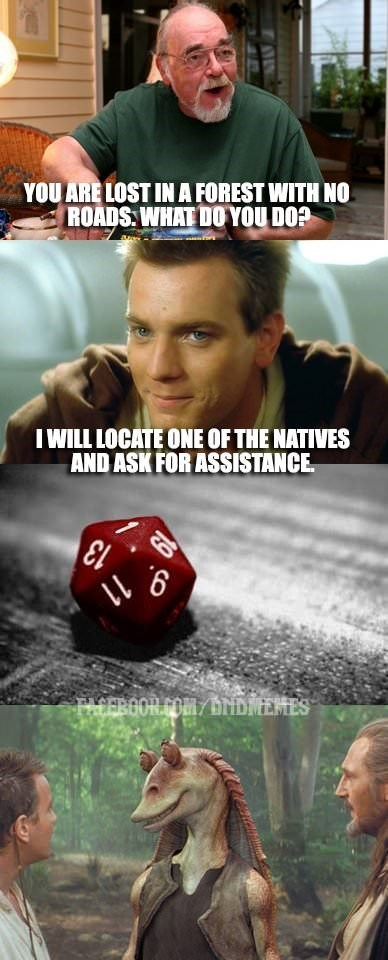
\includegraphics[width=0.3\textwidth]{images/jarjar.jpeg}
\end{center}

\end{frame}


\begin{frame}
\frametitle{Random Variable}

Looking at this from the perspective of application programmers, we say the number of users at time $t$ can be represented by a random variable $U$. 

Then we can ask ourselves what is the probability of $U$ being greater than 1000?

\end{frame}



\begin{frame}
\frametitle{Sample Space}

Probability is usually defined as some sort of experiment with sample space $\Omega$; some subset $E$ of $\Omega$ is an \alert{event}. (In full generality, sample spaces are measure spaces.)

A standard example: you have a perfectly fair coin. 

Possible outcomes are heads, tails, and very rarely, edge (it could happen). 

Each outcome is an event with a certain probability---i.e., chance of happening---usually written $P\{E_{n}\}$.


\end{frame}



\begin{frame}
\frametitle{Independence}

If the coin coming up heads is an event $E_{1}$ and it coming up tails $E_{2}$ are these independent? 

No, they are not. 

They are mutually exclusive---if the coin comes up heads it cannot possibly also come up tails. 


\end{frame}



\begin{frame}
\frametitle{Independence and Mutual Exclusivity}

Events are (measurable) sets and we can do unions and intersections and such. 

The formal definition of mutual exclusivity is $E_{1} \cap E_{2} = \emptyset$. 

Independence, on the other hand, means the probability of $E_{1}$ does not change if event $E_{2}$ has occurred.


\end{frame}



\begin{frame}
\frametitle{Conditional Probability}

Conditional probability is also important: what is the probability of event $E$ given that event $F$ has occurred? 

\begin{center}
	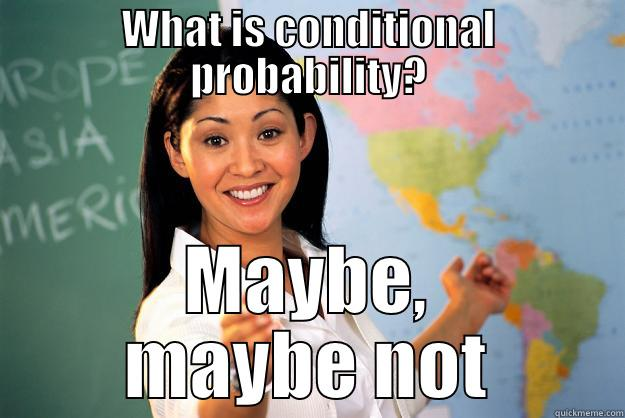
\includegraphics[width=0.4\textwidth]{images/conditional.jpg}
\end{center}

The notation is $P\{ E~|~F \}$ and it has a definition (as long as $P\{F\}$ is not zero): 

\begin{center}
	$P\{E~|~F\} = \dfrac{P\{E \cap F\}}{P\{F\}}$
\end{center}

\end{frame}



\begin{frame}
\frametitle{Independent Conditional}

If events $E$ and $F$ are independent, then $P\{E \cap F\}$ is equal to $P\{E\} \cdot P\{F\}$. 

That is, the probability of $E$ is not affected by the occurrence of $F$. 

Suppose you flip a coin four times and it comes up heads each time (event $F$). 

What is the probability that the next coin flip will be tails (event $E$)?

\end{frame}



\begin{frame}
\frametitle{Gambler's Fallacy}

Sadly, a lot of people think that after four heads, now tails is ``due'' and the chance of it being tails is higher than the usual 50-50 (minus the edge case)\footnote{Wikipedia will tell you about the Monte Carlo Casino in 1913.}.

This is not true---the next coin flip is independent of all the coin flips that went before it.

\end{frame}



\begin{frame}
\frametitle{Bayes Law}

If we want $P\{ F~|~E \}$, but have $P\{ E~|~F \}$ can we get it? 

Yes, if we know $P\{F\}$ and $P\{E\}$. 

Bayes law is:

\begin{center}
	$P\{F~|~E\} = \dfrac{P\{E~|~F\} \cdot P\{F\}}{P\{E\}}$
\end{center}


\end{frame}



\begin{frame}
\frametitle{Discrete Random Variables}


For now let us focus on discrete random variables (i.e., those with a countable number of values). 

For a random variable $X$ we can define a probability mass function (p.m.f.):

\begin{center}
	$p_{x}(a) = P \{ X = a \},$ where $\sum\limits_{x}^{~} p_{x}(x) = 1$
\end{center}
	and the cumulative distribution function is:
\begin{center}
	$F_{x}(a) = P \{ X \leq a \} = \sum\limits_{x \leq a} p_{x}(x)$
\end{center}


\end{frame}



\begin{frame}
\frametitle{There are Five Lights}

\begin{center}
	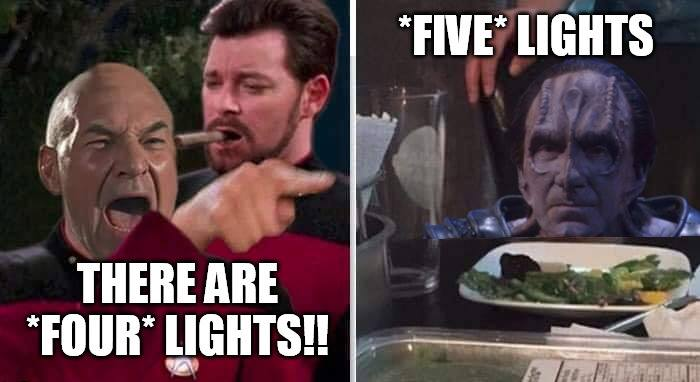
\includegraphics[width=0.4\textwidth]{images/fourlights.jpg}
\end{center}

There are five distributions we want to discuss: 

\begin{enumerate}
	\item Bernoulli 
	\item Binomial
	\item Geometric
	\item Poisson
	\item Exponential
\end{enumerate}

\end{frame}



\begin{frame}
\frametitle{Bernoulli}

Bernoulli represents a coin flip: so the coin has a probability $p$ of coming up heads and $1-p$ of coming up tails. 

So the random variable $X$ associated evaluates to 1 (heads) with probability $p$ and 0 (tails) with probability $1-p$. 

Thus the p.m.f. is $p_{x}(1) = p$ and $p_{x}(0) = 1 - p$. 

\end{frame}



\begin{frame}
\frametitle{Binomial}

The Binomial distribution builds upon the the Bernoulli distribution. 

A coin with probability $p$ of coming up heads flipped $n$ times (assuming coin flips are independent). 

The random variable $X$, if it's Binomial, represents the number of heads when flipping a Bernoulli coin $n$ times. 

So $X$ can take on values of $\{0, 1, ..., n\}$. 

\end{frame}



\begin{frame}
\frametitle{Geometric}

The Geometric distribution builds on Bernoulli. 

Again suppose we have the coin with probability $p$ of coming up heads. 

If we want to ask how many (independent) coin flips it will take until it comes up heads, the Geometric distribution answers this question. 

$X$ is the number of flips until we get the result we want.


\end{frame}



\begin{frame}
\frametitle{Examples in Computing}

Suppose we have a server farm that has $n$ disks, each of which independently dies (fails) with probability $p$ in a year. 

So what is the appropriate model for each of these questions?

\begin{enumerate}
	\item How many disks die in the first year?
	\item Given disk $d$, how long until this disk dies?
	\item After one year, is a specific disk $d$ alive or dead?
\end{enumerate}

\end{frame}



\begin{frame}
\frametitle{Computing Examples}

The answers are (1) Binomial, (2) Geometric, and (3) Bernoulli.

\end{frame}



\begin{frame}
\frametitle{Poisson}

Now let us turn to the Poisson distribution; this is very common in computing. 

This is our somewhat ``natural'' idea of randomness. 

This distribution arises when we have a mixture of a very large number of sources, each with a very small probability. 

So this is a lot like the number of arrivals to a website or packets at a router in some unit time. 

If a random variable $X$ has a Poisson distribution, the p.m.f. is:

\begin{center}
	$p_{x}(i) = \dfrac{e^{-\lambda}\lambda^{i}}{i!}$, where $i = 0, 1, 2....$
\end{center}

\end{frame}



\begin{frame}
\frametitle{Exponential}

We should also consider the exponential distribution. 

This is a distribution where the probability mass function (p.m.f.) drops off exponentially. 

If $x \geq 0$, then $f_{x}(x) = \lambda e^{-\lambda x})$. 

The cumulative distribution function, i.e., $F_{x}(x) = P\{ X \leq x \}$ is the integration of this function from negative infinity to $x$, equal to $1-e^{-\lambda x}$ (again, for $x \geq 0$). 

\end{frame}



\begin{frame}
\frametitle{Exponential}

What we care about here is actually the inverse of this, $\overline{F_{x}}(x)$, the probability that the value is greater than $x$.

These are the outliers or the ``tail'' of the distribution. 

Note that we see a constant drop-off of $e^{-\lambda}$ with each unit increase of $x$. 

Heavy tails are not very nice. 

\end{frame}



\begin{frame}
\frametitle{Expectation}

Recall the notation here $E[X]$ is the expected value of a random variable $X$. 

Expected value is, not kidding, just a ``weighted average''. 

Let's say you're entering into a game where you pay \$3 to play. 

If you have a 50\% chance of losing all your money, a 10\% chance of winning \$10, and a 40\% chance of getting your \$3 back, should you play?

\end{frame}



\begin{frame}
\frametitle{Gambling and ECON 101}

Do the math: your expected return is $(0.5 \times 0) + (0.1 \times 10) + (0.4 \times 3) \rightarrow 0 + 1 + 1.2 = 2.2$. 

So you expect that by playing this game, for every \$3 entry, you get back \$2.20 (on average). 

It doesn't seem like a good investment, does it? 

Econ 101 logic would tell you the answer is: how much do you value the fun of playing and the hope and excitement of winning? 

If it's equal to or more than \$0.80 then it is worth it.

\end{frame}



\begin{frame}
\frametitle{Proof by ``Because I Say So''}

Proofs of these exist in the textbook(s) but let's not belabour the point by proving it. 

Just take my word for it that the expectation for a Geometric distribution with probability $p$ is $1/p$.

If a Poisson distribution applies to something, the expectation $E[\lambda] = \lambda$.


\end{frame}



\begin{frame}
\frametitle{Variance}

The weighted average is nice, but it's not the whole story. 

If your numbers are 5, 6, and 7, then their average is 6. 

But the average of the numbers 0, 6, and 12 is also 6. 

But we should know already that averages can be misleading.

An average arrival rate of 1 request per second could still, with some probability, produce 3 arrivals in a single second.

\end{frame}



\begin{frame}
\frametitle{Variance}

The formal definition of variance of a random variable $X$ is the expected squared difference of $X$ from its mean:

\begin{center}
	$Var(X) = E[X^{2}] - (E[X])^{2}$
\end{center}


\end{frame}



\begin{frame}
\frametitle{Mean and Variance}

Just take my word for it at the moment that the following table is correct:

\begin{center}
\begin{tabular}{|l|l|l|}
	\hline
	\textbf{Distribution} & \textbf{Mean} & \textbf{Variance}\\ \hline
	Bernoulli & $p$ & $p(1-p)$\\ \hline
	Binomial & $np$ & $np(1-p)$\\ \hline
	Geometric & $\dfrac{1}{p}$ & $\dfrac{1-p}{p^{2}}$ \\ \hline
	Poisson & $\lambda$ & $\lambda$\\ \hline
\end{tabular}
\end{center}

\end{frame}



\begin{frame}
\frametitle{Convergence}

Think back to calculus class. 

Remember when we talk about limits: $\lim_{x\to\infty} f(x)$. 

%There is an answer for this if the function does (somehow) converge on some value, such as the function $f(x) = 1/x^{2}$ converging to 0.

\end{frame}



\begin{frame}
\frametitle{Random Variable Convergence}

We would like to see that our random variables converge. 

You might flip a coin four times and all four times it comes up heads. 

That doesn't match our expectation that we should have about half heads and half tails.

We have convergence if, given enough samples and enough sample paths, it will converge to the 0.5 we expect. 

\end{frame}


\begin{frame}
\frametitle{Stranger Things Have Happened...}

There may be sample paths that don't converge (e.g., continually coming up heads), but they have a ``probability mass'' of zero.

\begin{center}
	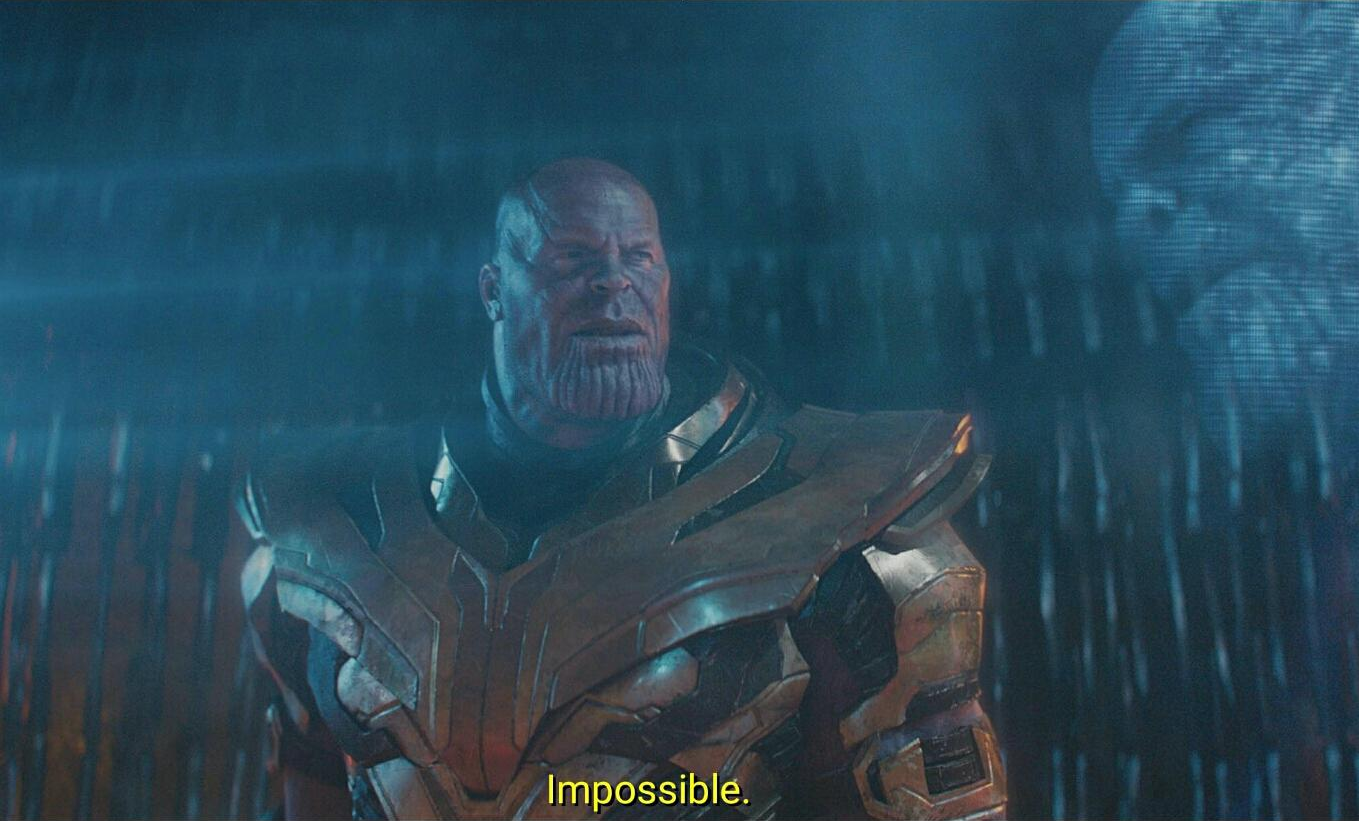
\includegraphics[width=0.4\textwidth]{images/thanos.png}
\end{center}

There are in fact uncountably many ``bad paths'', each with probability zero (but that's okay). Zero probability doesn't mean it can't happen, mind you.

\end{frame}



\begin{frame}
\frametitle{Convergence}

An image of what convergence looks like:

\begin{center}
	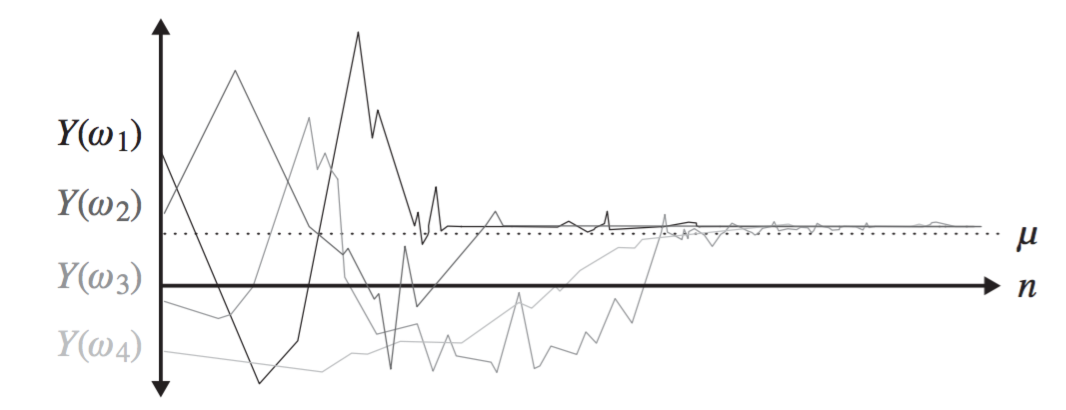
\includegraphics[width=0.6\textwidth]{images/convergence.png}
\end{center}

We won't concern ourselves with systems where there is no convergence. 

\end{frame}



\begin{frame}
\frametitle{Tim and Enzo}

A small but important digression on the subject of sampling, measurement, and testing.

You have an idea of what an average is, but there are two different types of average---the time average and ensemble average. 


\end{frame}



\begin{frame}
\frametitle{Tim and Enzo Scenario}

Let us just focus on having a single First-Come-First-Serve queue. 

Every second, a new job arrives with probability $p$ and if there is any work to do, the job being worked on is completed with probability $q$ (and $q > p$). 

As a definition, let $N(v)$ equal the number of jobs in the system at a time $v$. 

In the story, Tim and Enzo are trying to simulate the FCFS system to determine what is the average number of jobs in the system.

\end{frame}



\begin{frame}
\frametitle{The Tim Approach}

Tim decides he's going to run it as one really long simulation. 

He simulates the queue over a very long period, logging as he goes, taking a million samples. 

Then he takes the average value over those samples to get the average number of jobs.

\end{frame}



\begin{frame}
\frametitle{The Enzo Approach}

Enzo does something slightly different: instead of having one super long simulation, he does 1000 shorter simulations. 

He waits until the simulation has run for 1000 seconds and then samples the queue at exactly that point, obtaining one value. 

This experiment is restarted with a new random seed. 

So after obtaining a thousand samples, he averages these, and Enzo produces another average number of jobs.


\end{frame}



\begin{frame}
\frametitle{Tim and Enzo}

\begin{center}
	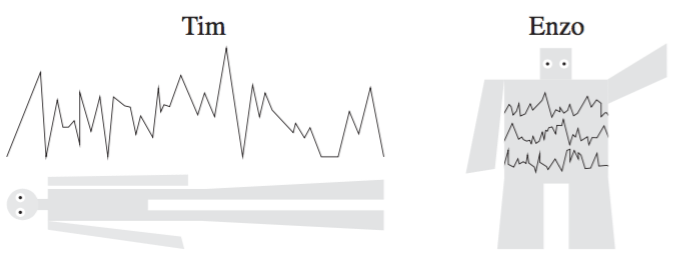
\includegraphics[width=0.8\textwidth]{images/timenzo.png}
\end{center}

So---who has done this correctly, Tim or Enzo?

\end{frame}



\begin{frame}
\frametitle{Time Average vs Ensemble Average}

The time average has potential problems because we are only looking at a single sequence and maybe something very unusual has happened here in this single run. 

The ensemble average is more likely what we talk about when we talk about the system being at ``steady state'' (i.e., past the initial conditions). 

So we kind of like the Enzo approach. Tim's approach still has some merit though.

\end{frame}



\begin{frame}
\frametitle{Initial Conditions}

Both the Tim and Enzo approaches here require caring about the initial conditions. 

Enzo needs to make sure that the initial conditions (startup costs etc) have attenuated before the measurement point. 

Tim needs to ensure that the initial conditions impact a sufficiently small portion of all his measurements.

\end{frame}



\begin{frame}
\frametitle{Everyone's a Winner}

If we have a nicely behaved system, the time average and the ensemble average are the same (so both Tim and Enzo can be correct). 

What is a nicely behaved system? The word for this is \alert{ergodic}. 

That probably did not help, so what is an ergodic system? 

It is a system that is positive recurrent, aperiodic, and irreducible.

\end{frame}



\begin{frame}
\frametitle{Irreducibility}

\alert{Irreducibility} means a process should be able to get from one state to any other state (where state is the number of jobs in the system). 

This means the initial state of the system does not matter. 

So if we started at 0 jobs or 10 we could still get to any state in the system (jobs at 2 or 27)...

\end{frame}



\begin{frame}
\frametitle{Positive Recurrence}

\alert{Positive recurrence} means that given an irreducible system, any state $i$ is revisited infinitely often, and the time between visits to that state are finite. 

So we can define a certain state as being a ``restart''. 

The logical choice in the case of a queue or similar is the idea of the queue being empty. 

Every time the queue gets down to zero jobs, it's a ``restart'' of sorts. 

\end{frame}



\begin{frame}
\frametitle{Positive Recurrence}

This is what makes Tim's view and Enzo's view potentially the same. 

A single long run (Tim's view) is just like a number of independent runs (Enzo's view). 

Every time we get down to zero jobs in the queue, it's a restart. 

\end{frame}



\begin{frame}
\frametitle{Aperiodicity}

The \alert{aperiodicity} condition is required for the ensemble average to make sense or exist. 

That is to say, the state of the system should not be related to the the time.

Otherwise the way Enzo chooses to sample, i.e., $t = 1000$, is potentially going to skew the result.

\end{frame}



\begin{frame}
\frametitle{Tim as Enzo}

\begin{center}
	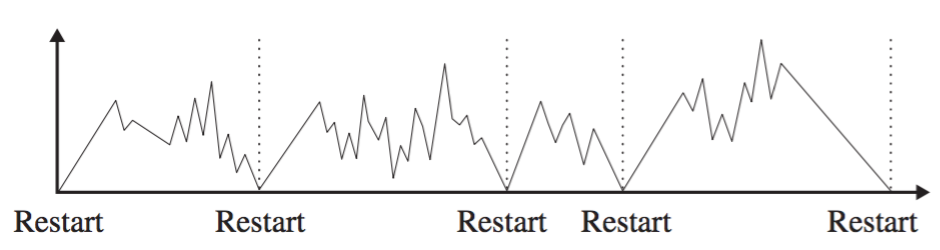
\includegraphics[width=0.8\textwidth]{images/systemrestart.png}
\end{center}

So both Tim and Enzo are correct, given an ergodic system.


\end{frame}



\begin{frame}
\frametitle{How Long Jobs Are in the System}

We could compute either the time or ensemble average. 

\begin{center}
	Time Average = $\lim_{t\to\infty}\dfrac{\sum_{i=1}^{A(t)} T_{i}}{A(t)}$
\end{center}

where $A(t)$ is the number of arrivals by time $t$ and $T_{i}$ is the time in the system of arrival $i$. The average is taken over one sample path.


\end{frame}

\begin{frame}
\frametitle{How Long Jobs Are in the System}

\begin{center}
	Ensemble Average = $\lim_{t\to\infty}E[T_{i}]$
\end{center}

where $E[T_{i}]$ is the average time in the system of job $i$, where the average is taken over all sample paths.


\end{frame}

\end{document}

